\documentclass{article}

\usepackage{../preamble}
\standalonetrue

\pagestyle{fancy}
\fancyhf{}
\rhead{Section \thesection}
\lhead{PHYS 304 Lecture 17}
\rfoot{Page \thepage}


\title{PHYS 304 Lecture 17}
\author{Ashtan Mistal}
\date{!!!}

\begin{document}

\ifstandalone
\maketitle
\fi

\graphicspath{{./Lecture17/}}


\section{Brief overview of last class}

\begin{itemize}
    \item By expanding the expectation value of some operator of some observable in the basis defined by the set of eigen states of that same operator, it is clear that the probability of measuring a particular eigen value of that operator is proportional to the squared magnitude of the projection of the state of interest on that eigen state.  The generalized statistical interpretation is that if you carry out a measurement of that observable, with sufficient resolution, you must measure one of the eigen values, and the state will be collapsed after the measurement to the corresponding eigen state (discrete spectrum language, must tweak for continuous spectrum).
    
    \item The derivation of the generalized uncertainty relationship between the variances of any two physical observables $A$, and $B$, for a system in a particular state, is technically straight forward, and the product of the variances is proportional to the squared amplitude of the expectation value of the commutator of $\hat{A}$ and $\hat{B}$. We used $[\hat{A}, \hat{B}]$ as a shorthand for $\hat{A} \hat{B} - \hat{B} \hat{A}$.  
    
    $$\sigma_A^2 \sigma_B^2 \geq \left( \frac{1}{2i} \braket{\left[ \hat{A}, \hat{B} \right]} \right)^2$$
    
    \item We showed that $[\hat{x}, \hat{p}] = i \hbar \hat{I}$ regardless of $V(x)$, using the differential operators in position space, acting on an arbitrary wavefunction in position space. 
    
    \item We showed that $[\hat{p}, \hat{E}] = [\hat{p}, \frac{\hat{p}}{2m}] = 0$ for a free particle, regardless of what state it operates on, so that $\sigma_p^2 \sigma_E^2 \geq 0$ for a free particle (it can be arbitrarily close to 0). 
    
    \item We further showed that $[\hat{p}, \hat{E}] = [\hat{p}, \frac{\hat{p}^2}{2m} + \frac{k}{x} \hat{x}^2] = -i\hbar k \braket{\hat{x}}$ for a particle in a harmonic potential $V(x) = \frac{1}{2}kx^2$, and thus $\sigma_p^2 \sigma_E^2 \geq \frac{\hbar^2}{4} k^2 \braket{\hat{x}}^2$ for a particle in a harmonic potential. The product of variances in this case is state-dependent.  

\end{itemize}

\section{Today: Finishing chapter 3}

\begin{itemize}
    \item Some interpretation of the generalized uncertainty relation
    \item The energy-time uncertainty relation
\end{itemize}

\subsection{Discussion}

Fundamentally, the generalized uncertainty relation we derived imposes a constraint on the product of variances one would deduce by making several measurements of the exact same state $\ket{S(t)}$ at some time $t$, first in one observable, and then in another observable (or randomly measuring one of the two variables many times).  

\begin{itemize}
    \item It does NOT imply anything, in general, about the product of those variances at any other time
    \item It does NOT imply anything, directly, about what happens if you try to measure two quantities at the same time (a very complicated process, in general).
    \item The constraint IS an \textbf{inequality}, NOT an equality!
\end{itemize}

\hfill

Some further reading if you're interested:

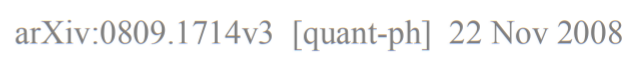
\includegraphics[width = 0.5 \textwidth]{Lecture17/1.png}

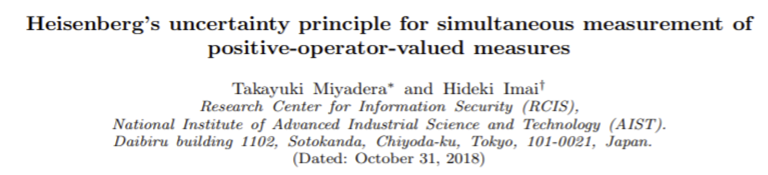
\includegraphics[width = 0.5 \textwidth]{Lecture17/2.png}

Poll: Which of the following statements follows what we have learned about the uncertainty principle so far? 

\begin{itemize}
    \item If two observables share the same set of eigen states, the variance of measurements of at least one of those observables must be zero for a particle in any state (T/\textbf{F})
    \item If two observables share the same set of eigen states, it is possible that there are states for which repeated measurements of each observable would result in arbitrarily small variance in both measurements (\textbf{T}/F)
    \item If the commutator of two observables is proportional to the identity operator, it is impossible to find a state in which the variance in the measurement of one observable is arbitrarily small (T/\textbf{F}) % measure with infinite precision (arbitrarily precise precision)
    \item The minimum value of the product of variances for two observables for a particle in some state must be independent of time (T/\textbf{F}) %counterexample: momentum and energy in the harmonic oscillator potential
    \item \textbf{If two operators do not commute, and their commutator is state-independent, if you try to manufacture a state that has very small variance in one of the observables, then as you decrease that variance, the variance of the other observable must increase (\textbf{T}/F)}

\end{itemize}


\subsection{Minimum uncertainty state}

$$\sigma_x \sigma_p \geq \frac{\hbar}{2}$$

What satisfies the equality condition (the "minimum uncertainty state"?)

\textit{see text Section 3.5.2 for discussion / derivation}

$$\psi(x) = Ee^{\left\{ -a (x \langle x \rangle)^2 \right\}} e^{(i \langle p \rangle \frac{x}{\hbar}}$$

where $\braket{x}$ and $\braket{p}$ are real constants. 

Is this familiar? 

This is our old Gaussian wavepacket!

What happens if we make $\hat{A} = \hat{E} = \hat{H}$?

$$\sigma_H^2 \sigma_B^2 \geq \left( \frac{1}{2i} \braket{[\hat{H}, \hat{B}]} \right)^2$$

We will now show that the expectation value of the commutator of any time-independent operator, call it $\hat{B} = \hat{Q}$  with the total energy operator, is related to the time derivative of the expectation value of the operator $\hat{Q}$. Thus we seek a simplification of the following:

$$\sigma_H^2 \sigma_Q^2 \geq \left( \frac{1}{2i} \braket{[\hat{H}, \hat{Q}]} \right)^2$$

under the constraint that $\langle \frac{\partial}{\partial t} \hat{Q} \rangle = 0$. \textbf{NOTE:} $\langle \frac{\partial}{\partial t} \hat{Q} \rangle \neq \frac{d}{dt} \langle \hat{Q} \rangle$. 

This is a subtle but very important distinction!

\subsection{Simplification}

\begin{enumerate}
    \item Expand $\frac{d}{dt} \braket{\hat{Q}}$
    
    Assume:
    
    \begin{itemize}
        \item $\hat{Q}$ is independent of time
    \end{itemize}
    
    $$\frac{d}{dt} \braket{Q} = \frac{d}{dt} \braket{S(t)|\hat{Q}|S(t)} = \frac{\partial \bra{S(t)}}{\partial t} \left( \hat{Q} \ket{S(t)} \right) + \braket{S(t)| \left( \underbrace{\frac{\partial \hat{Q}}{\partial t}}_{=0} \right)|S(t)} + \bra{S(t)} \hat{Q} \left( \frac{\partial}{\partial t} \ket{S(t)} \right)$$
    
    SE in immutable Hilbert space:
    
    $$\frac{\partial \ket{S(t)}}{\partial t} = \frac{-i}{\hbar} \hat{H} \ket{S(t)} \Rightarrow \frac{\partial \bra{S(t)}}{\partial t} = \frac{i}{\hbar} \bra{S(t)} \hat{H}^+ = \frac{i}{\hbar} \bra{S(t)} \hat{H}$$
    
    $$\Rightarrow \frac{d}{dx} \braket{Q} = \frac{i}{\hbar} \braket{S(t)|\hat{H} \hat{Q} | S(t)} - \frac{i}{\hbar} \braket{S(t)|\hat{Q} \hat{H}|S(t)}$$
    
    $$= \frac{i}{\hbar} \braket{S(t)| \left[ \hat{H}, \hat{Q} \right] |S(t)} = \frac{i}{\hbar } \langle \left[ \hat{H}, \hat{Q} \right] \rangle$$
    
    So, 
    
    $$\frac{d}{dt} \braket{\hat{Q}} = \frac{i}{\hbar} \braket{[\hat{H}, \hat{Q}]} + \sigma_H^2 \sigma_Q^2 \geq \left( \frac{1}{2i} \braket{\left[ \hat{H}, \hat{Q} \right]} \right)^2$$
    
    $$\sigma_H^2 \sigma_Q^2 \geq \left( \frac{1}{2i} \frac{\hbar}{i} \frac{d \braket{\hat{Q}}}{dt} \right)^2$$
    
    $$\sigma_H^2 \sigma_Q^2 \geq \frac{\hbar}{2} |  \frac{d \braket{\hat{Q}}}{dt}|$$
    
    
    \item Use the fact that $\frac{\partial}{\partial t} \ket{S(t)} = \frac{-i}{\hbar} \hat{H} \ket{S(t)}$, and our constraint that $\langle \frac{\partial}{\partial t} \hat{Q} \rangle = 0$
\end{enumerate}

Finally:

% insert slide 11

What does this tell us?


The direct, or fundamental connection between the generalized uncertainty relation and the energy-time uncertainty relation is through the proportionality of the product of the variances of the energy operator and any other Hermitian operator, with the rate of change of the expectation value of the Hermitian operator of interest. 

The variance in the energy of some state at any given time must be greater than or equal to the normalized rate of change of any Hermitian observable in that state.  

Let's ponder these results:

\begin{itemize}
    \item a) The variance in the energy of a state at some particular time depends on the other observable with which you might be comparing variances. (T/\textbf{F})
    \item b) If the variance of the energy of a state at some particular time is very small, then the normalized rate at which any observable can vary at that time must be very slow.  (\textbf{T}/F) \footnote{This makes sense with the notion of a "stationary state"}
    \item c) If any observable has a very fast normalized rate of change at some particular time, then the variance of the energy at that time must be very large. (\textbf{T}/F)

\end{itemize}

% copy slide 14

% copy slide 15

% copy slide 16


\section{Extra Question}

Is the statement: "A quantum state contains all the info one can ever know about a system" only valid for \textbf{closed} systems?

\begin{itemize}
    \item The short answer is yes. 
\end{itemize}

However, please note that the vectors $\ket{S(t)} \in H_{Hilbert}$ that we are familiar with are only valid for closed systems anyways. 

If you go to \textbf{open} systems, the concept of a quantum state is generalized to a \textbf{density matrix}. If you have access to the open system only, the this density matrix will in fact again contain all the info you can possibly get from it. However, if you have knowledge about the surroundings, then you can get more info about the open system. However, do note that this new information will be contained the combined state of the (open system + surrounding). 

%see diagram that Arnab shared with me




\end{document}